\documentclass[letterpaper,12pt,oneside]{article}
\usepackage[top=1in, left=1.25in, right=1.25in, bottom=1in]{geometry}
\usepackage{setspace}
\usepackage{float} % Coloca esto en el preámbulo de tu documento

\usepackage[T1]{fontenc}
\usepackage[utf8]{inputenc}
\usepackage[spanish,es-nodecimaldot,es-tabla]{babel}
\usepackage{caption, subcaption} %figuras
\usepackage{graphicx}
\usepackage{array}
\usepackage{tikz}
\usepackage{imakeidx}
\usepackage{biblatex}
\addbibresource{protocolo.bib}

\graphicspath{{./images1/}}
\usepackage[none]{hyphenat}
\linespread{1.5}
\usepackage{ragged2e}

\begin{filecontents}{protocolo.bib}
@online{cisco_router_2023,
    author = {Cisco},
    title = {What is a router?},
    year = {2023},
    url = {https://www.cisco.com/c/es_mx/solutions/small-business/resource-center/networking/what-is-a-router.html#~how-does-a-router-work},
    urldate = {2024-09-07}
}

@online{cloudflare_router_sf,
    author = {Cloudflare},
    title = {What is a Router?},
    url = {https://www.cloudflare.com/learning/network-layer/what-is-a-router/},
    urldate = {2024-09-07}
}

@online{nordvpn_mascara_2024,
    author = {NordVPN},
    title = {¿Qué es una máscara de subred y para qué sirve?},
    year = {2024},
    url = {https://nordvpn.com/es-mx/blog/que-es-mascara-de-subred/},
    urldate = {2024-09-07}
}

@online{kaspersky_ip_2024,
    author = {Kaspersky},
    title = {¿Qué es una dirección IP?},
    year = {2024},
    url = {https://latam.kaspersky.com/resource-center/definitions/what-is-an-ip-address},
    urldate = {2025-09-13}
}

@online{todoelectronica_switch_2023,
    author = {Todo Electronica},
    title = {Guía completa sobre los Switch de red y conexiones CCTV},
    year = {2023},
    url = {https://www.todoelectronica.com/blog-electronica/guia-completa-sobre-los-switch-de-red-conexiones-cctv.html},
    urldate = {2025-09-13}
}

@online{ppstech_switch_2024,
    author = {PPS-Tech},
    title = {¿Cómo funciona un switch? Una pieza clave para empresas},
    year = {2024},
    url = {https://ppstech.mx/blog/como-funciona-un-switch-una-pieza-clave-para-empresas},
    urldate = {2025-09-13}
}

@online{studysmarter_ieee_sf,
    author = {StudySmarter},
    title = {Protocolos IEEE},
    url = {https://www.studysmarter.es/resumenes/ingenieria/ingenieria-de-telecomunicaciones-ingenieria/protocolos-ieee},
    urldate = {2025-09-13}
}
\end{filecontents}

\begin{document}

	% ----------------- PORTADA -----------------
	% ----------------- PORTADA -----------------
	\begin{titlepage}
		\centering
		
		% Escudo de la UNAM
		\vspace*{0cm}  % Reduce espacio arriba
		
\includegraphics[width=3cm]{../images1/UNAM_LOGO2.png}\par
		\vspace{0.1cm}   % Ajuste espacio debajo del escudo
		
		{\Large \textbf{Universidad Nacional Autónoma de México} \par}
		\vspace{0.1cm}
		{\large \textbf{Facultad de Estudios Superiores Aragón} \par}
		\vspace{0.1cm}
		{\large \textbf{Ingeniería en Computación} \par}
		
		\vspace{0.1cm}  % Ajuste menor
		
		{\LARGE \textbf{Redes de Computadoras} \par}
		\vspace{0.2cm}
		{\Large \textbf{Práctica 1} \par}
		
		\vspace{0.3cm}  % Ajuste para espacio antes de los datos
		
		% Bloque de Alumno, Grupo, Semestre
		\begin{center}  
			\large
			\textbf{Alumno:} \\[0.2cm]
			320009336 \\[0.2cm]
			320076628 \\[0.2cm]
			320084225 \\[0.2cm]
			320272105 \\[0.2cm]
			423040368 \\[0.2cm]
			
			\textbf{Grupo:} \\[0.2cm]
			8701 \\[0.2cm]
			
			\textbf{Semestre:} \\[0.2cm]
			2026-II
		\end{center}
		
		\vspace{0.2cm}  % Espacio antes de la fecha
		
		{\large México, CDMX. Septiembre 2025 \par}
		
	\end{titlepage}
	
	% ----------------- ÍNDICE MANUAL -----------------
	\newpage
	\begin{center}
		{\LARGE \textbf{Índice}}
	\end{center}
	\vspace{1cm}
	
	\begin{flushleft}
		\textbf{1. Introducción} \hfill \textbf{2} \\[0.5cm]
		\textbf{2. Marco Teórico} \hfill \textbf{4} \\[0.5cm]
		\textbf{3. Desarrollo} \hfill \textbf{6} \\[0.5cm]
		\textbf{4. Resultados} \hfill \textbf{11} \\[0.5cm]
		\textbf{5. Conclusiones} \hfill \textbf{16} \\[0.5cm]
        \textbf{6. Bibliografía} \hfill \textbf{17} \\[0.5cm]
	\end{flushleft}
\clearpage

\section{Introducción}
\subsection*{Planteamiento del problema}
En el contexto de las redes de computadoras, la configuración y la interconexión de dispositivos son tareas esenciales en entornos domésticos tanto como empresariales. Este reporte aborda la simulación de dos escenarios de red básicos: el primero, el establecimiento de una red local (LAN) utilizando un switch, y el segundo, la comunicación entre diferentes clases de red a través de un router. El problema radica en cómo configurar correctamente los dispositivos finales y los intermediarios para asegurar la conectividad y el flujo de datos entre ellos. La práctica se enfoca en resolver este problema a través de la configuración de direcciones IP y la utilización de los dispositivos de interconexión adecuados, todo ello simulado en Cisco Packet Tracer.

\subsection*{Motivación}
La práctica es esencial para el desarrollo profesional como estudiantes de ingeniería en computación. Los conceptos de redes no son meramente teóricos; su aplicación práctica es lo que permite construir infraestructuras de comunicación funcionales. Este ejercicio es una oportunidad para consolidar los conocimientos sobre direccionamiento IP, clases de red y el rol de los dispositivos de capa 2 (switch) y capa 3 (router). Al dominar estas habilidades básicas, se sientan las bases para el diseño, la implementación y la resolución de problemas en redes complejas en futuros proyectos y en el entorno laboral real.

\subsection*{Objetivos}
El principal objetivo de esta práctica es comprender y aplicar los conceptos de interconexión de redes mediante la simulación. Se busca lograr los siguientes objetivos específicos:
\begin{itemize}
    \item Configurar una red con un switch: Modelar y configurar una LAN con un switch y cinco computadoras, asignando direcciones IP de la clase C y verificando la conectividad de los dispositivos.
    \item Configurar una red con un router: Establecer comunicación entre tres computadoras que pertenecen a diferentes clases de red (A, B y C) utilizando un router, y comprender la importancia del cable cruzado en este tipo de conexión.
    \item Utilizar herramientas de diagnóstico: Emplear las herramientas de Cisco Packet Tracer, como el comando \texttt{ping} y la función de entorno de mensaje, para validar que la configuración de la red es exitosa y que la comunicación entre los dispositivos se lleva a cabo correctamente.
\end{itemize}
\clearpage

\section{Marco Teórico}
\subsection*{¿Qué es un router?}
Es un dispositivo que sirve de punto de conexión entre una red local e Internet. Los routers gestionan, o enrutan, el tráfico web y los datos entre dispositivos de diferentes redes, y permiten que varios dispositivos compartan la misma conexión a Internet.

\subsection*{¿Qué es una IP y una máscara de subred?}
Una dirección IP es como la \textit{dirección física de tu casa} en el mundo real, pero para tu computadora en una red. Es un número único que identifica a tu dispositivo y permite que la información (paquetes de datos) sepa a dónde debe ir. Por ejemplo, cuando navegas por una página web, tu computadora envía una solicitud a la dirección IP del servidor de esa página para que te envíe los datos. La máscara de subred es como un \textit{código postal} o una clave que le dice a tu computadora qué parte de su dirección IP identifica a la red a la que pertenece y qué parte identifica al dispositivo dentro de esa red. Para seguir con la analogía de la casa, la máscara de subred ayuda a distinguir si la dirección de otra computadora está en tu misma calle (la misma red local) o si está en otra ciudad (una red externa).

\subsection*{¿Qué es un switch?}
Un switch de red es un dispositivo utilizado en redes de computadoras para conectar múltiples dispositivos y permitir la comunicación entre ellos. Actúa como un punto central de conexión para enviar datos entre los aparatos conectados; como computadoras, impresoras, cámaras de seguridad, etc. El switch analiza las direcciones MAC (Media Access Control) de los dispositivos conectados y envía los datos al destino correcto.

\subsection*{¿Qué son los protocolos de comunicación IEEE?}
Los protocolos IEEE son estándares desarrollados por el Instituto de Ingenieros Eléctricos y Electrónicos, fundamentales para asegurar la interoperabilidad y calidad de dispositivos electrónicos y de comunicación. Un ejemplo famoso es el IEEE 802.11, que regula las redes inalámbricas Wi-Fi, facilitando conexiones estables y seguras alrededor del mundo. Estos protocolos resultan esenciales para la evolución de tecnologías emergentes, garantizando eficiencia y compatibilidad en sistemas de telecomunicaciones globales.

\subsection*{Gateway (Puerta de Enlace)}
El gateway es un dispositivo (generalmente un router) que sirve como punto de entrada y salida de una red. Cuando un dispositivo en una red local necesita comunicarse con un dispositivo en una red externa, envía los datos al gateway, que se encarga de reenviarlos a su destino. Es la dirección IP que los dispositivos finales utilizan para salir de su red local.

\subsection*{Cableado de Red}
Existen dos tipos principales de cables de red Ethernet:
\begin{itemize}
    \item Cable directo (Straight-through): Conecta dispositivos diferentes, como un PC a un switch. Los hilos en ambos extremos del cable están conectados en el mismo orden.
    \item Cable cruzado (Crossover): Conecta dispositivos del mismo tipo, como un PC a otro PC, o un switch a otro switch. Los hilos de transmisión de un extremo están cruzados con los hilos de recepción del otro extremo, lo que permite la comunicación. En la práctica, el router se conecta a los PCs con cable cruzado para permitir la comunicación entre redes de clases diferentes.
\end{itemize}
\clearpage

\section{Desarrollo}
\subsection*{Topología 1}
En la primera topología, el objetivo principal fue configurar una red local (LAN) mediante la instalación y conexión de dispositivos a un switch. Cisco Packet Tracer, al ser un simulador didáctico, permite observar cómo se construye y administra la red en un entorno controlado sin necesidad de hardware físico (Cisco Networking Academy, 2022).

\textbf{Instalación y configuración del switch:}
Se colocó un \texttt{empty switch} al cual se le agregaron cinco puertos Fast Ethernet. Para realizar esta operación, el dispositivo debía estar en estado \texttt{off} para evitar conflictos en la instalación de módulos. Esta etapa resulta relevante ya que, en la vida real, los switches permiten ampliar la capacidad de conexión en redes LAN, centralizando la comunicación de múltiples dispositivos.
\begin{figure}[h!]
    \centering
    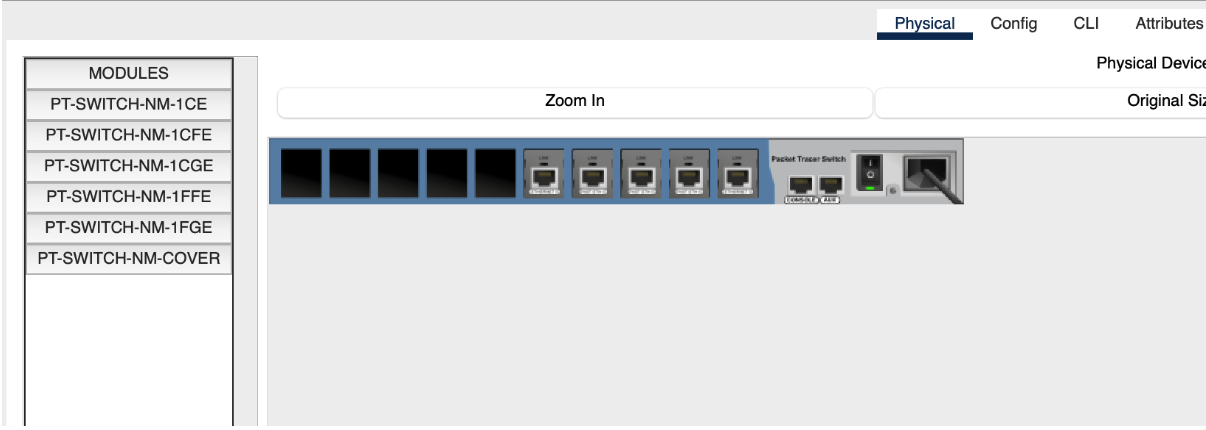
\includegraphics[width=0.9\textwidth]{1.png}
\end{figure}

\textbf{Asignación de la puerta de enlace predeterminada (default gateway):}
Se configuró el valor 192.168.1.254 como puerta de enlace. Aunque en una LAN el switch no siempre actúa como \texttt{gateway}, en este caso se asignó este valor para fines de simulación y coherencia en la práctica, asegurando que los dispositivos tuvieran un parámetro de referencia común para la salida de datos.
\begin{figure}[h!]
    \centering
    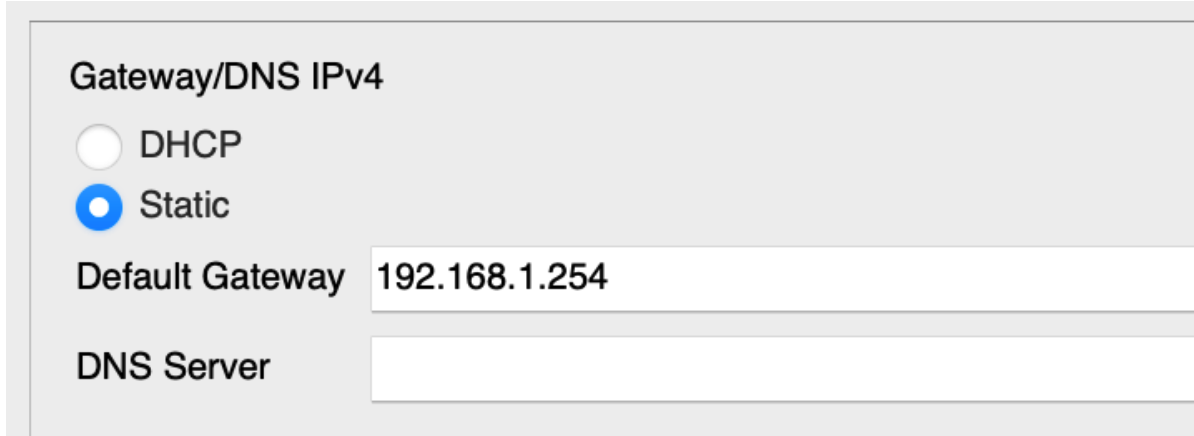
\includegraphics[width=0.9\textwidth]{2.png}
\end{figure}

\textbf{Conexión de los equipos terminales:}
Se añadieron cinco computadoras (PCs), conectadas al switch mediante cables de cobre directo. El sistema indicó su correcta conexión a través de los triángulos verdes, confirmando el estado operativo de las interfaces de red. En la práctica real, este indicador equivaldría a verificar los LEDs de actividad en los puertos de un switch físico.
\begin{figure}[h!]
    \centering
    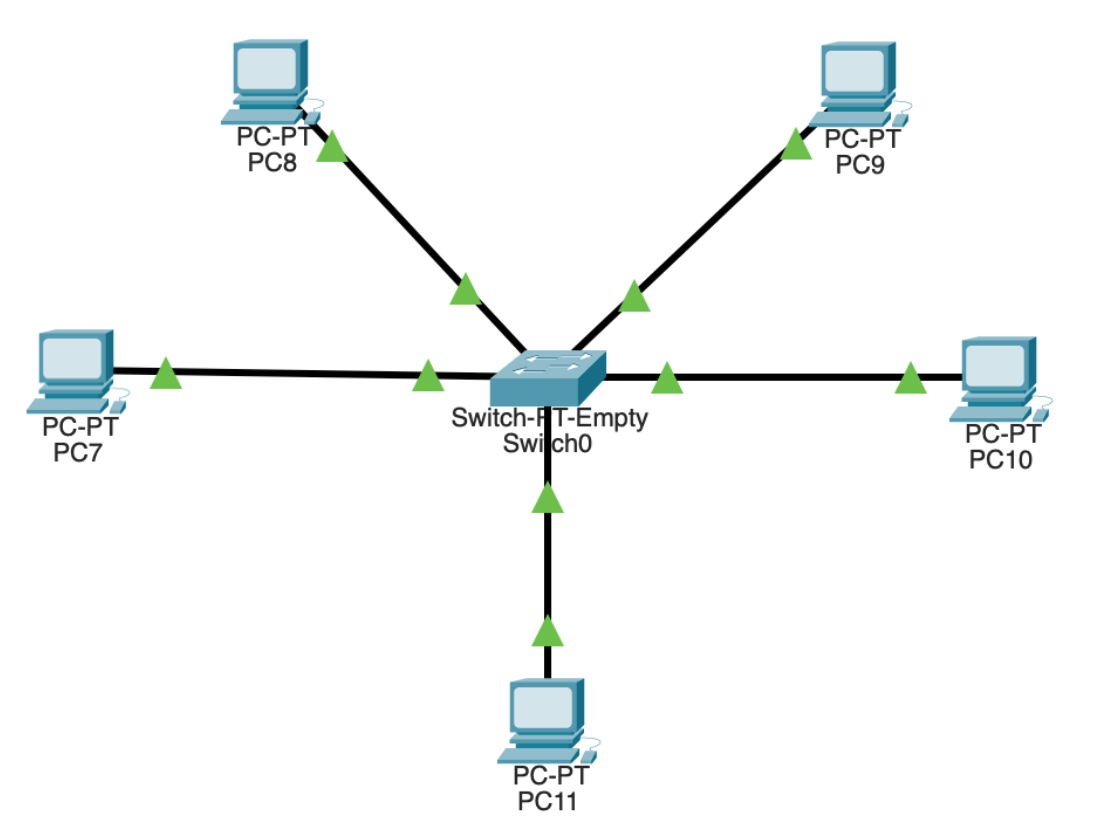
\includegraphics[width=0.9\textwidth]{3.png}
\end{figure}

\textbf{Configuración de direcciones IP y máscaras de subred:} A cada computadora se le asignó una dirección IP única dentro del rango de la red, junto con la máscara 255.255.255.0, asegurando que pertenecieran al mismo dominio de broadcast. Asimismo, se configuró el \texttt{default gateway} con el valor 192.168.1.254, garantizando homogeneidad en la red.
\begin{itemize}
    \item PC1 $\rightarrow$ IP: 192.168.1.1, Gateway: 192.168.1.254
    \item PC2 $\rightarrow$ IP: 192.168.1.2, Gateway: 192.168.1.254
    \item PC3 $\rightarrow$ IP: 192.168.1.3, Gateway: 192.168.1.254
    \item PC4 $\rightarrow$ IP: 192.168.1.4, Gateway: 192.168.1.254
    \item PC5 $\rightarrow$ IP: 192.168.1.5, Gateway: 192.168.1.254
\end{itemize}
\begin{figure}[h!]
    \centering
    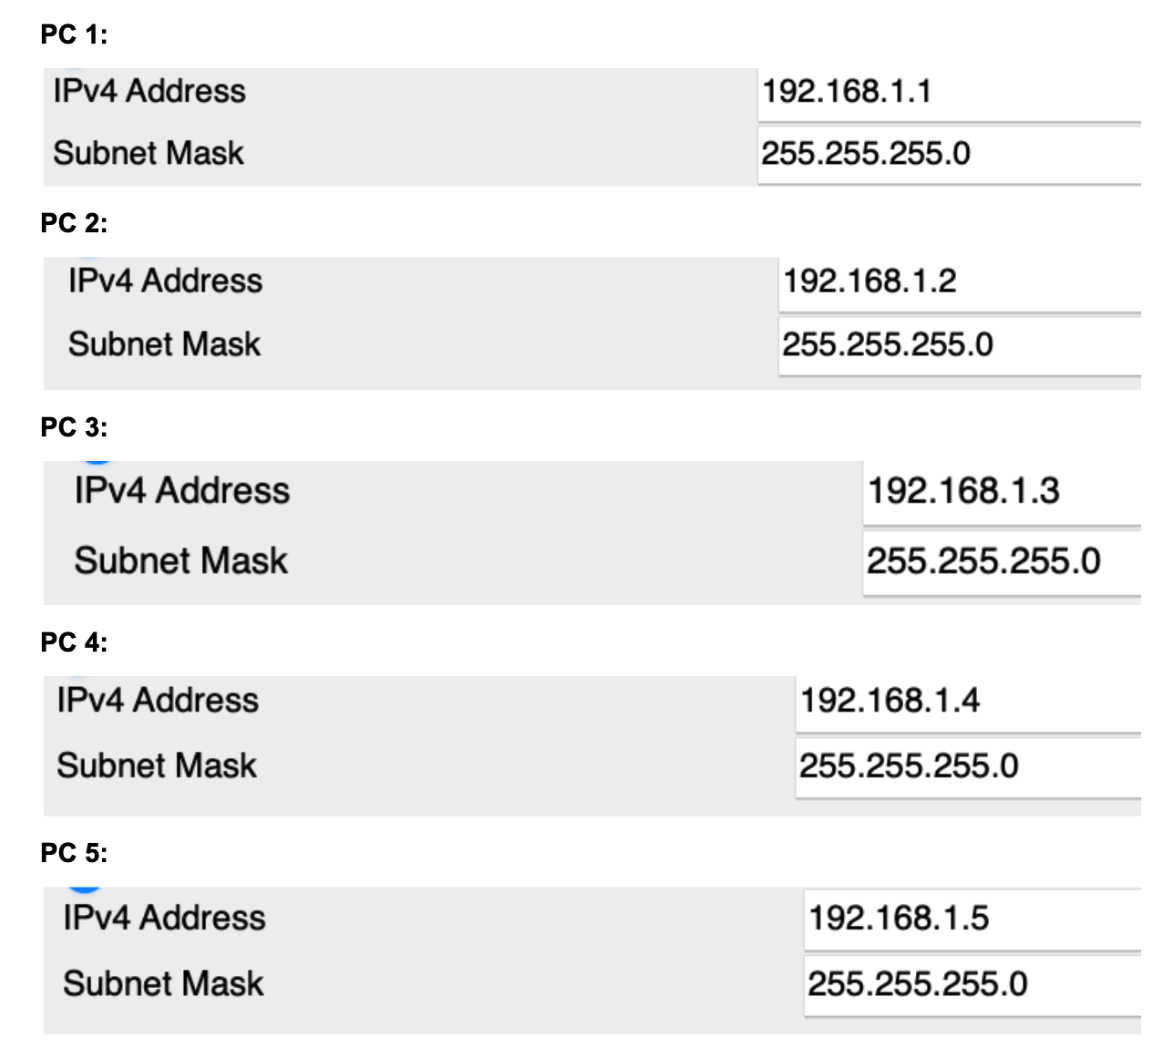
\includegraphics[width=0.9\textwidth]{4.png}
\end{figure}

\subsection*{Topología 2: Red Segmentada con Router}
La segunda topología planteó un escenario más complejo, ya que los dispositivos terminales se encontraban separados en diferentes segmentos de red. Esto implica la necesidad de un router, dispositivo encargado de interconectar redes con distintos esquemas de direccionamiento IP.
\begin{figure}[h!]
    \centering
    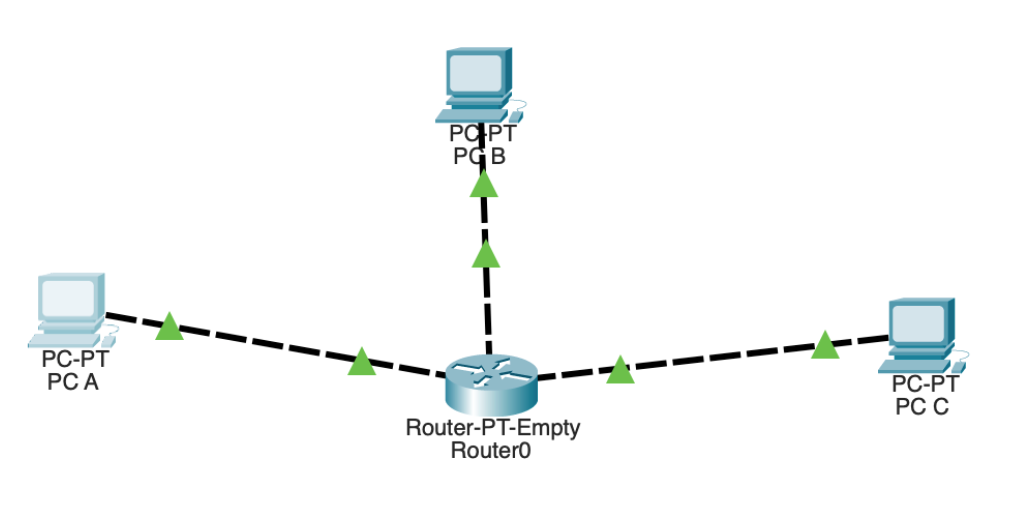
\includegraphics[width=0.9\textwidth]{11.png}
\end{figure}

\textbf{Instalación del router y sus interfaces:}
Se colocó un router vacío y se le instalaron puertos Fast Ethernet. A diferencia del switch, que trabaja en la Capa 2 del modelo OSI (capa de enlace de datos), el router opera en la Capa 3 (red), lo que le permite tomar decisiones de enrutamiento basadas en direcciones IP.
\begin{figure}[h!]
    \centering
    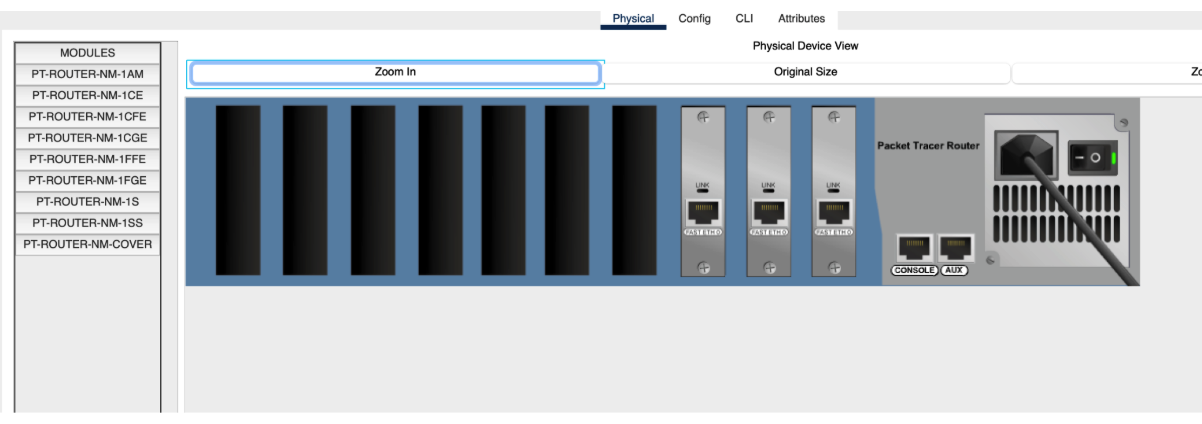
\includegraphics[width=0.9\textwidth]{12.png}
\end{figure}

\textbf{Conexión de los segmentos mediante cables cruzados:}
Dado que el router y las PCs se encuentran en el mismo nivel de jerarquía, se emplearon cables cruzados (crossover). Esta elección responde a la regla clásica de conexión en redes, donde dispositivos similares requieren un cable cruzado, mientras que dispositivos distintos se interconectan con un cable directo.


\textbf{Asignación de direcciones IP y gateways en cada segmento:} Cada segmento de la red fue configurado con una dirección de red distinta, lo que garantiza la segmentación lógica y evita conflictos de direccionamiento:
\begin{itemize}
    \item Segmento A:
    \begin{itemize}
        \item IP PC A: 10.0.0.1
        \item Gateway: 10.0.0.254
    \end{itemize}
    \item Segmento B:
    \begin{itemize}
        \item IP PC B: 172.16.0.1
        \item Gateway: 172.16.0.254
    \end{itemize}
    \item Segmento C:
    \begin{itemize}
        \item IP PC C: 192.168.1.1
        \item Gateway: 192.168.1.254
    \end{itemize}
\end{itemize}
\begin{figure}[h!]
    \centering
    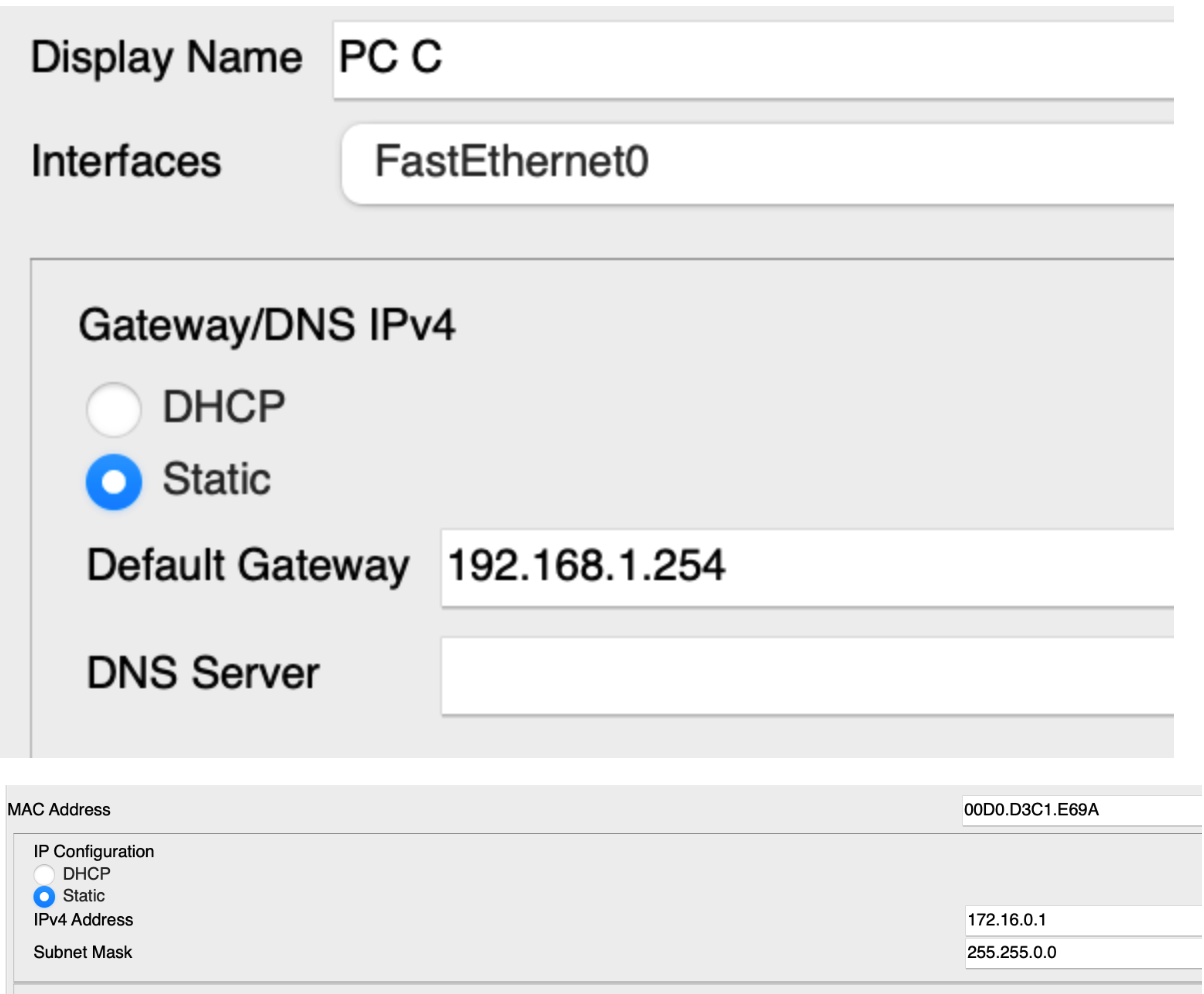
\includegraphics[width=0.9\textwidth]{18.png}
\end{figure}
\clearpage

\section{Resultados}
Se revisó si la comunicación y la conexión era correcta entre todos los dispositivos, ya sea de dispositivo a switch, switch a equipo o de equipo a equipo.
\begin{figure}[h!]
    \centering
    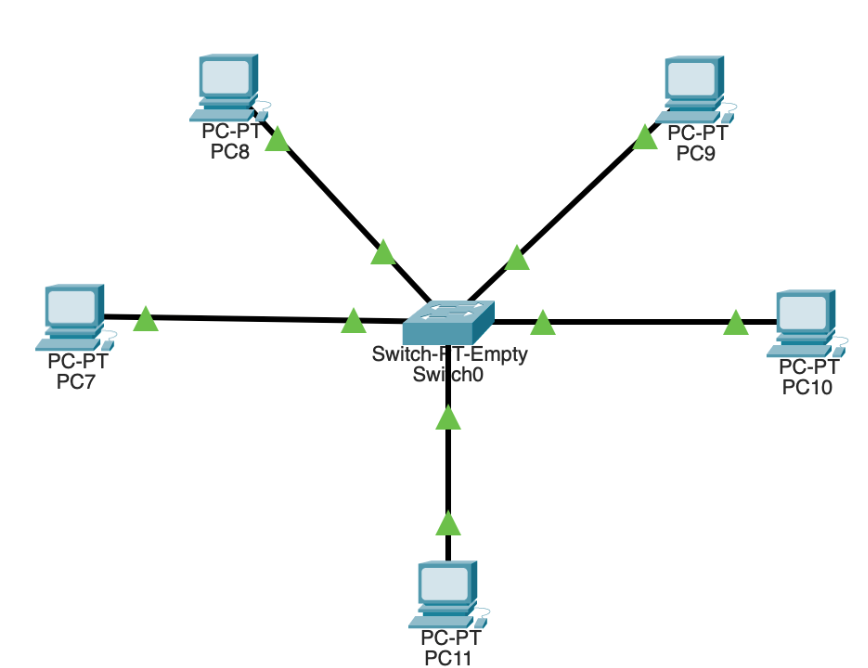
\includegraphics[width=0.9\textwidth]{19.png}
\end{figure}

\textbf{Verificación de la comunicación:}

Para validar la configuración, se realizaron simulaciones con el ícono de la carta, que permiten visualizar gráficamente el recorrido de los paquetes de datos. En las tres pruebas realizadas, se obtuvo un 100\% de éxito, lo cual confirma que los parámetros de red fueron correctamente aplicados.

\begin{figure}[H]
\centering
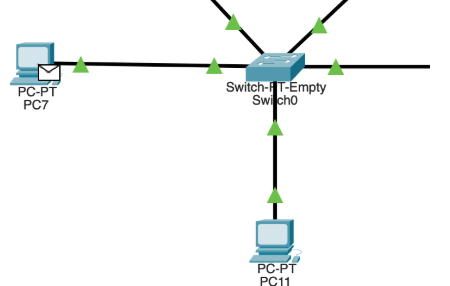
\includegraphics[width=0.9\textwidth]{20.png}
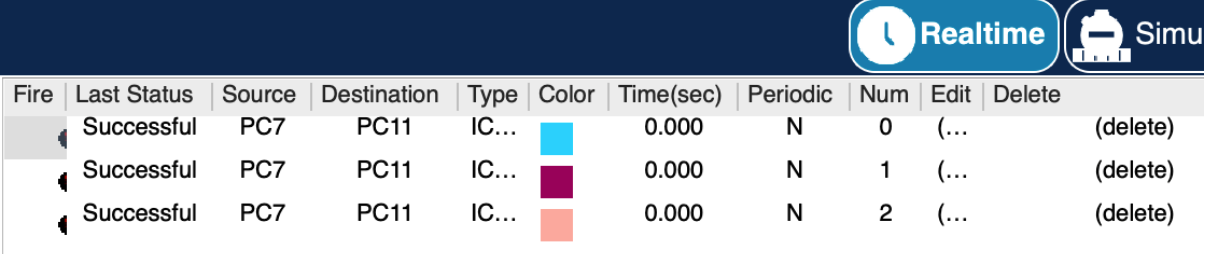
\includegraphics[width=0.9\textwidth]{21.png}
\caption{Imágenes 20 y 21: Verificación de la comunicación}
\end{figure}

\textbf{Pruebas con herramientas de diagnóstico:} 

Se utilizó la herramienta \texttt{Command Prompt} de cada PC, desde la cual se ejecutó el comando \texttt{ping} hacia las demás direcciones IP. Esta verificación mostró la respuesta con tiempos de latencia mínimos, lo que indica conectividad eficiente. Según Forouzan (2017), el comando \texttt{ping} es una de las formas más simples y efectivas para comprobar si un dispositivo es alcanzable dentro de una red IP. Con esta primera topología se comprobó la importancia de la configuración uniforme de parámetros de red y de la correcta conexión física, elementos que garantizan la comunicación en una LAN básica.

\begin{figure}[H]
\centering
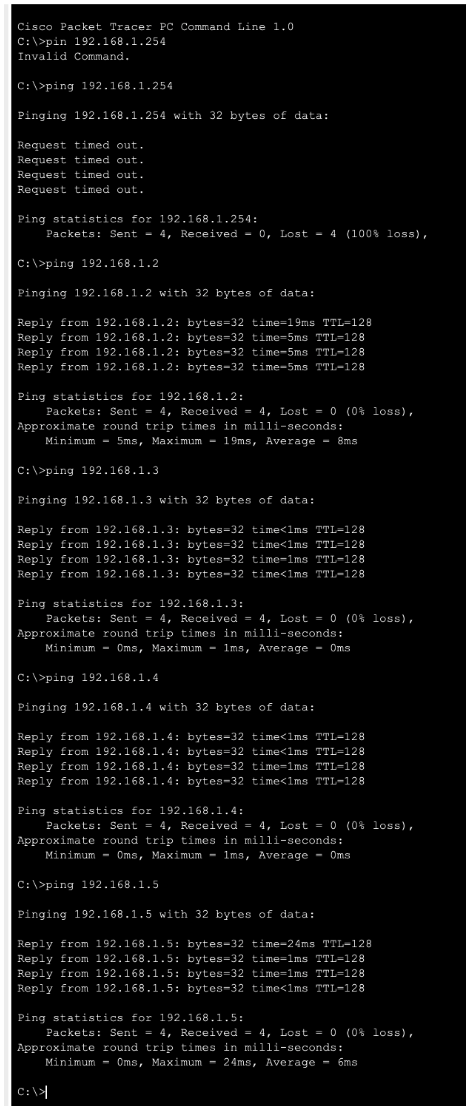
\includegraphics[width=0.6\textwidth]{22.png}
\caption{Imagen 22: Escalada de pruebas de diagnóstico}
\end{figure}

\textbf{Simulación y validación de la comunicación:}

Al ejecutar la simulación con el ícono de la carta, se observó que los paquetes atravesaban exitosamente el router, lo que confirma que este cumplía con la función de intermediario entre subredes. Además, se ejecutaron pruebas con el comando \texttt{ping}, confirmando la conectividad entre los tres segmentos y mostrando los tiempos de respuesta de cada intercambio.

\begin{figure}[H]
\centering
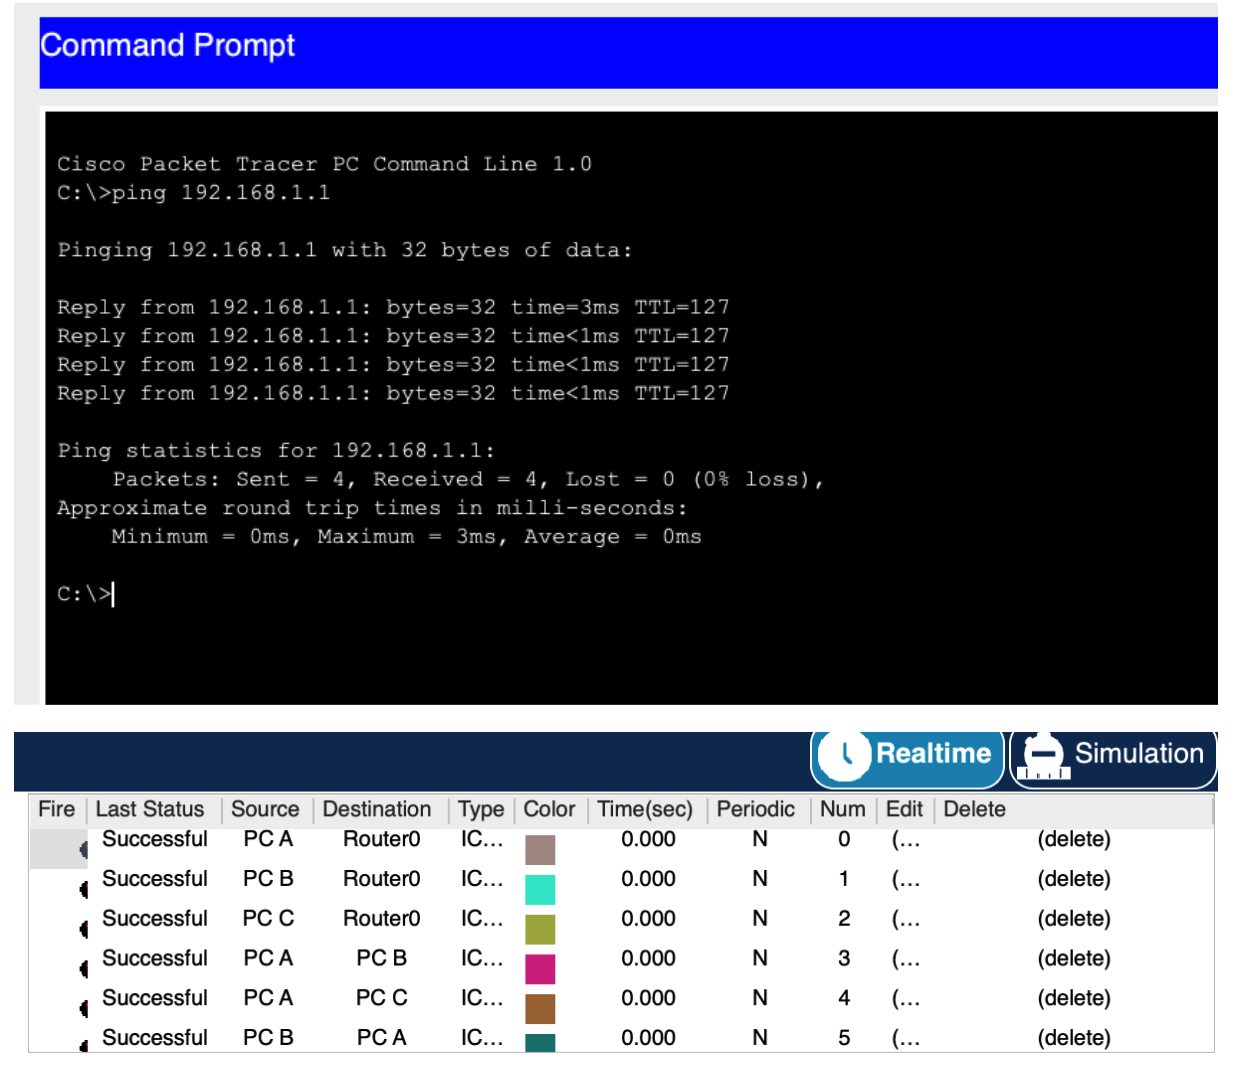
\includegraphics[width=0.9\textwidth]{23.png}
\caption{Imagen 23: Simulación y validación de la comunicación}
\end{figure}

\textbf{Relevancia de redes:}
La práctica demostró que el router no solo interconecta distintas redes, sino que también actúa como dispositivo de control y filtrado de tráfico, ya que cada interfaz puede configurarse con políticas de acceso y protocolos de enrutamiento. De acuerdo con Tanenbaum y Wetherall , "los routers son la columna vertebral de Internet, al permitir la interconexión entre millones de redes privadas y públicas".
\begin{figure}[H]
\centering
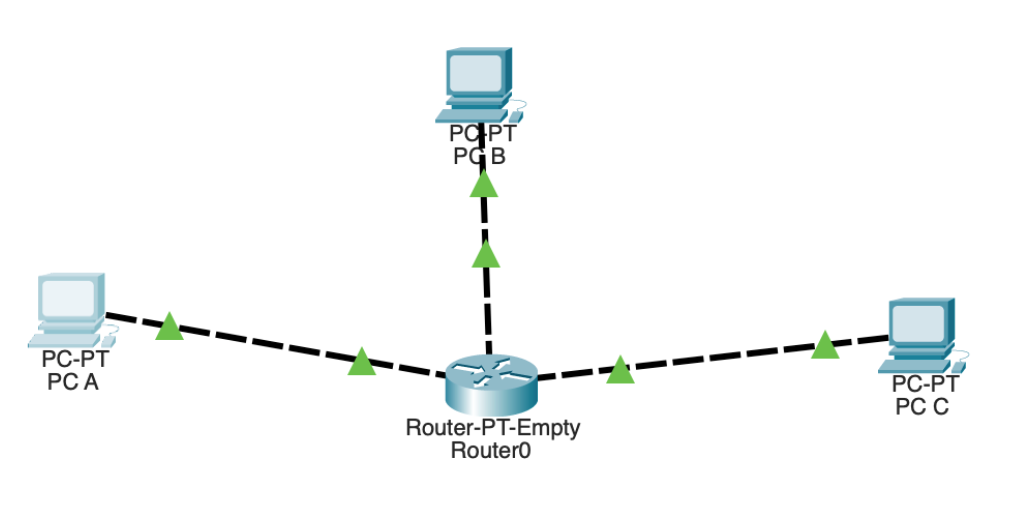
\includegraphics[width=0.9\textwidth]{11.png}
\caption{Imagen 11: Relevancia de redes}
\end{figure}



\clearpage

\section{Conclusiones}
El desarrollo de la práctica cumplió satisfactoriamente con los objetivos planteados en la introducción: comprender la configuración de redes locales mediante switch y la interconexión de distintos segmentos de red con router. Desde la motivación inicial, orientada a reconocer la importancia de la comunicación digital en nuestra vida cotidiana y profesional, se logró constatar cómo los fundamentos de dirección IP, máscaras de subred y dispositivos de interconexión resultan indispensables para garantizar una conectividad eficiente.
\begin{itemize}
    \item En el primer escenario, se alcanzó el objetivo de crear una red LAN básica que demostrara la función del switch como dispositivo centralizador en la capa 2. La práctica evidenció que, al configurar adecuadamente las direcciones IP y las puertas de enlace, la comunicación entre equipos se establece de manera fluida y confiable.
    \item En el segundo escenario, se cumplió el objetivo de comprender el papel de los routers en la segmentación y enrutamiento de redes. La configuración realizada mostró cómo es posible conectar diferentes subredes y garantizar la comunicación entre ellas mediante el uso de gateways.
\end{itemize}
Las motivaciones iniciales, que destacaban la necesidad de adquirir competencias técnicas aplicables tanto en el ámbito académico como en el profesional, se vieron plenamente reflejadas en los resultados. La práctica no solo facilitó la asimilación de conocimientos abstractos, sino que también brindó herramientas de diagnóstico y resolución de problemas, esenciales en escenarios reales. En conclusión, esta actividad contribuyó a consolidar competencias técnicas básicas en redes y evidenció la importancia de la práctica para complementar la teoría.
\clearpage

\section*{Bibliografía}
\begin{itemize}
    \item Cisco. (2023). \textit{What is a router?}. Recuperado de \url{https://www.cisco.com/c/es_mx/solutions/small-business/resource-center/networking/what-is-a-router.html#~how-does-a-router-work}. Consultado el 07 de septiembre de 2024.
    \item Cloudflare. \textit{What is a Router?}. Recuperado de \url{https://www.cloudflare.com/learning/network-layer/what-is-a-router/}. Consultado el 07 de septiembre de 2024.
    \item NordVPN. (2024). \textit{¿Qué es una máscara de subred y para qué sirve?}. Recuperado de \url{https://nordvpn.com/es-mx/blog/que-es-mascara-de-subred/}. Consultado el 07 de septiembre de 2024.
    \item Kaspersky. (2024). \textit{¿Qué es una dirección IP?}. Recuperado de \url{https://latam.kaspersky.com/resource-center/definitions/what-is-an-ip-address}. Consultado el 13 de septiembre de 2025.
    \item Todo Electronica. (2023). \textit{Guía completa sobre los Switch de red y conexiones CCTV}. Recuperado de \url{https://www.todoelectronica.com/blog-electronica/guia-completa-sobre-los-switch-de-red-conexiones-cctv.html}. Consultado el 13 de septiembre de 2025.
    \item PPS-Tech. (2024). \textit{¿Cómo funciona un switch? Una pieza clave para empresas}. Recuperado de \url{https://ppstech.mx/blog/como-funciona-un-switch-una-pieza-clave-para-empresas}. Consultado el 13 de septiembre de 2025.
    \item StudySmarter. (s.f.). \textit{Protocolos IEEE}. Recuperado de \url{https://www.studysmarter.es/resumenes/ingenieria/ingenieria-de-telecomunicaciones-ingenieria/protocolos-ieee}. Consultado el 13 de septiembre de 2025.
\end{itemize}

\end{document}